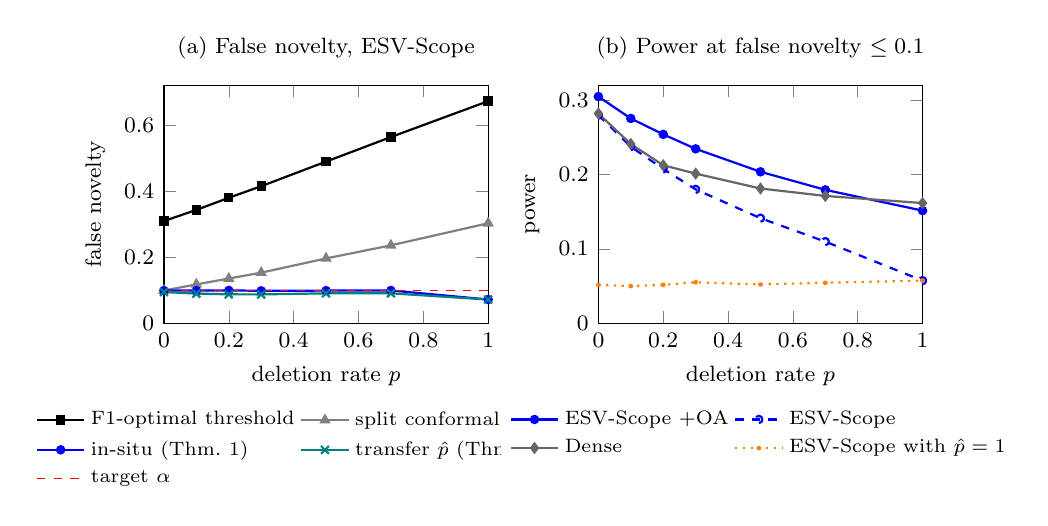
\begin{tikzpicture}
\begin{axis}[name=left, width=0.47\textwidth, height=4.6cm, xmin=0, xmax=1, ymin=0, ymax=0.72,
  xlabel={deletion rate $p$}, ylabel={false novelty}, label style={font=\footnotesize},
  tick label style={font=\footnotesize}, title={(a) False novelty, ESV-Scope}, title style={font=\footnotesize},
  legend style={font=\scriptsize, at={(0.5,-0.32)}, anchor=north, legend columns=2, draw=none},
  legend cell align=left]
\addplot[thick, black, mark=square*, mark size=1.3pt] coordinates {(0,0.3092) (0.1,0.3429) (0.2,0.3796) (0.3,0.4147) (0.5,0.4892) (0.7,0.5636) (1,0.6723)};
\addplot[thick, gray, mark=triangle*, mark size=1.6pt] coordinates {(0,0.0987) (0.1,0.1172) (0.2,0.1350) (0.3,0.1528) (0.5,0.1959) (0.7,0.2355) (1,0.3024)};
\addplot[thick, blue, mark=*, mark size=1.3pt] coordinates {(0,0.0987) (0.1,0.0984) (0.2,0.0990) (0.3,0.0978) (0.5,0.0984) (0.7,0.0989) (1,0.0714)};
\addplot[thick, teal, mark=x, mark size=2pt] coordinates {(0,0.0940) (0.1,0.0894) (0.2,0.0871) (0.3,0.0869) (0.5,0.0901) (0.7,0.0902) (1,0.0714)};
\addplot[dashed, red, domain=0:1, samples=2] {0.1};
\legend{F1-optimal threshold, split conformal (complete), in-situ (Thm.~1), transfer $\hat p$ (Thm.~2), target $\alpha$}
\end{axis}
\begin{axis}[at={(left.east)}, anchor=west, xshift=1.4cm, width=0.47\textwidth, height=4.6cm, xmin=0, xmax=1, ymin=0, ymax=0.32,
  xlabel={deletion rate $p$}, ylabel={power}, label style={font=\footnotesize},
  tick label style={font=\footnotesize}, title={(b) Power at false novelty $\le 0.1$}, title style={font=\footnotesize},
  legend style={font=\scriptsize, at={(0.5,-0.32)}, anchor=north, legend columns=2, draw=none},
  legend cell align=left]
\addplot[thick, blue, mark=*, mark size=1.3pt] coordinates {(0,0.3050) (0.1,0.2755) (0.2,0.2541) (0.3,0.2346) (0.5,0.2037) (0.7,0.1794) (1,0.1514)};
\addplot[thick, blue, dashed, mark=o, mark size=1.3pt] coordinates {(0,0.2799) (0.1,0.2376) (0.2,0.2075) (0.3,0.1800) (0.5,0.1412) (0.7,0.1097) (1,0.0572)};
\addplot[thick, black!60, mark=diamond*, mark size=1.6pt] coordinates {(0,0.2821) (0.1,0.2411) (0.2,0.2125) (0.3,0.2013) (0.5,0.1812) (0.7,0.1712) (1,0.1616)};
\addplot[thick, orange, dotted, mark=star, mark size=1.6pt] coordinates {(0,0.0516) (0.1,0.0499) (0.2,0.0515) (0.3,0.0550) (0.5,0.0520) (0.7,0.0543) (1,0.0572)};
\legend{ESV-Scope +OA, ESV-Scope, Dense, ESV-Scope with $\hat p=1$}
\end{axis}
\end{tikzpicture}
